\chapter{Conversores CC com Cargas de Potência Constante} \label{cap3}

\section{Microrredes de Corrente Contínua}

No século XX, a "Guerra das Correntes" entre defensores da \acrshortpl{ca}, liderados por \textit{Westinghouse} e \textit{Tesla}, e proponentes da \acrshort{cc}, liderados por \textit{Edison}, resultou na prevalência da \acrshort{ca} devido à sua facilidade de expansão da rede. Apesar disso, a \acrshort{cc} permaneceu relevante com os avanços na eletrônica de potência. Paralelamente, a crescente adoção de microrredes \acrshortpl{cc}, com \acrfullpl{fer}, \acrfullpl{sae} e novas cargas, reflete das preocupações ambientais e escassez de combustíveis fósseis, mas sua integração descoordenada apresenta desafios técnicos e operacionais, como perfil de tensão comprometido e congestionamentos nas linhas de transmissão. \cite{Elsayed2015, Dragicevic2015}.

A proposta das \acrshortpl{mr} surgiu como uma solução há mais de uma década. As \acrshortpl{mr} operando em modo isolado ou conectadas à rede, podem ser classificadas como \acrshortpl{mr} de \acrshort{ca} ou \acrshort{cc}. Devido à sua maior eficiência e melhor interface com diversos tipos de \acrshort{fer} e \acrshort{sae}, a s\acrshortpl{mr} de \acrshort{cc}, cuja estrutura básica está representada na \autoref{fig:microgrid}, é mais atraente. Além disso, ao serem acopladas em torno de um barramento \acrshort{cc}, as \acrshortpl{mr} eliminam problemas como fluxo de potência reativa e regulação de frequência, resultando em sistemas de controle menos complexos. \cite{Dragicevic2015}.

\begin{figure}[H]
  \centering
  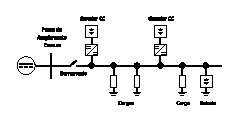
\includegraphics[width=0.87\textwidth]{figuras/microgrid.eps}
  \caption{Estrutura básica de uma microrrede.}
  \label{fig:microgrid}
\end{figure}

Vários setores empregam \acrfullpl{sdcc}, como espaçonaves, centros de dados, telecomunicações, tração e sistemas de energia a bordo de navios. Por exemplo, a Estação Espacial Internacional utiliza \acrshortpl{sdcc} para operar suas vastas necessidades de energia. Alguns centros de dados também adotaram sistemas \acrshort{cc}, resultando em economia significativa de energia em comparação com sistemas \acrshort{ca} tradicionais. Na área de telecomunicações, os sistemas de distribuição de energia de 48V são amplamente empregados para garantir alta confiabilidade e eficiência. Além disso, sistemas de tração, como bondes e metrôs, preferem distribuição \acrshort{cc} devido à facilidade de interface com motores \acrshort{cc}. Esses sistemas também permitem maior eficiência e controlabilidade. Em sistemas de energia a bordo de navios, a distribuição zonal \acrshort{cc} é uma opção popular devido à sua confiabilidade e facilidade de proteção. \cite{Elsayed2015}.

Desta forma, o design de sistemas de distribuição \acrshort{cc} tem recebido atenção crescente, especialmente devido a adaptação de equipamentos projetados originalmente para \acrshort{ca}. Modelos simplificados são essenciais para compreender o comportamento da carga em operação \acrshort{cc}. Comparando configurações de cabos, descobriu-se que sistemas \acrshort{cc} podem superar \acrshort{cc} em termos de capacidade de transferência de energia, \cite{Salomonsson2007}. Em um estudo sobre microrredes \acrshort{cc} em centros de dados, \cite{Salomonsson2008}, foi proposto um sistema de controle adaptativo para otimizar o fluxo de energia e minimizar perdas. Essas pesquisas contribuem para uma compreensão mais profunda do design e controle de sistemas de distribuição DC.

% MR: Conversores e CPLs - Introdução
Os conversores \acrshort{cc}-\acrshort{cc} são dispositivos bastante utilizados para regular a tensão nas \acrshortpl{mr} \acrshort{cc}, facilitando a integração de fontes de energia renovável e tradicional. Contudo, grande quantidades de conversores conectados nas \acrshortpl{mr} \acrshort{cc} pode afetar a estabilidade do sistema. Além disto, estes conversores podem energizar \acrfullpl{cpl}, cujo circuito equivalente está descrito na figura a seguir:

\begin{figure}[H]
  \centering
  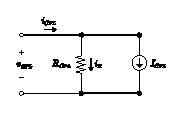
\includegraphics[width=0.4\textwidth]{figuras/cpl_circuit.eps}
  \caption{Circuito simplificado de uma CPL.}
  \label{fig:cpl_circuit}
\end{figure}

\noindent A partir deste circuito, pode-se derivar a seguinte equação dinâmica: \begin{equation} i_{\text{CPL}}(t) = i_R(t) + I_{\text{CPL}} = \frac{P_{\text{CPL}}}{(v_{\text{CPL}}(t))^2} + I_{\text{CPL}} \label{eq:cpl-circuit},\end{equation} onde $P_{\text{CPL}}$ representa a potência da \acrshort{cpl}. Ao linearizar a equação dinâmica \eqref{eq:cpl-circuit} em torno do ponto de operação $P_0$ para a potência da \acrshort{cpl} e $V_0$ para a tensão da \acrshort{cpl}, pode-se obter a seguinte expressão: \begin{equation} \delta i_{\text{CPL}}(t) = - \frac{P_0}{{V_0}^2}\delta v_{\text{CPL}}(t) + I_{\text{CPL}}. \end{equation} Considerando que $\frac{1}{R_0} = - \frac{P_0}{{V_0}^2}$, é possível observar a presença de uma impedância negativa e, da equação \eqref{eq:cpl-circuit}, a não linearidade da \acrshort{cpl}. Estas característica podem causar oscilações indesejadas que podem causar instabilidade e colapso do sistema das \acrshortpl{mr}. \cite{Bessa2020, Amiri2020}.

% MR: Soluções Propostas
Para resolver esses problemas, foram propostas várias técnicas de controle, incluindo filtros RL ou RC, controle preditivo, técnicas robustas, o uso de resistência virtual e métodos de controle não lineares, como controle de modo deslizante e controle preditivo de modelo. O desenvolvimento de controladores robustos e observadores de distúrbios é comum para manter a estabilidade, com o método de backstepping considerado particularmente eficaz. No entanto, desafios adicionais surgem devido à incerteza nos parâmetros do conversor e distúrbios associados aos \acrshortpl{cpl}, exigindo abordagens mais sofisticadas de controle e análise de estabilidade. \cite{Bessa2020, Amiri2020}.

\section{Conversores \acrshort{cc}-\acrshort{cc}}

Os conversores \acrshort{cc}-\acrshort{cc} são circuitos que transferem energia elétrica de uma fonte de entrada para uma de saída. Estes conversores operam por meio de semicondutores que atuam como interruptores, controlando o fluxo de energia através de elementos passivos, como indutores e capacitores. O variável fundamental para determinar a operação do conversor é a razão cíclica, ou ciclo de trabalho, que define a proporção de tempo em que os interruptores permanecem ligados e desligados. Entre as diversas topologias de conversores \acrshort{cc}-\acrshort{cc}, destacam-se os conversores Buck e Boost, que serão abordados neste trabalho.

\subsection{Conversor Buck} \label{section:buck_converter}

% Buck: Introdução
O conversor \acrshort{cc}-\acrshort{cc} abaixador de tensão, mais conhecido como conversor Buck, produz uma tensão de saída média menor que a entrada. Isso ocorre devido à conservação de energia, resultando em uma corrente de saída média maior que a corrente de entrada média. Teoricamente, o conversor Buck permite uma variação contínua da tensão na carga, de zero até a tensão de entrada. \cite{martins2008}.

% Buck: Configuração Básica
A configuração básica do conversor Buck é apresentada na \autoref{fig:basic-buck-converter}.

\begin{figure}[H]
  \centering
  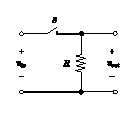
\includegraphics[width=0.27\textwidth]{figuras/basic_buck_conversor.eps}
  \caption{Configuração básica do conversor Buck.}
  \label{fig:basic-buck-converter}
\end{figure}

% Buck: Valor médio de tensão
O valor médio da tensão da carga, $\bar{v}_{out}$ é descrito como: \begin{equation} \bar{v}_{out} = \frac{t_c}{T}v_{in}, \end{equation} onde, $t_c$ é o tempo em que a chave $S$ permanece fechada, $t_a$ é o tempo em que a chave permanece aberta, e $T = t_c + t_a$ é o período de chaveamento. \cite{martins2008}.

% Buck: parâmetros do circuito
A razão cíclica, ou duty cycle, é definida como: \begin{equation} d = \frac{t_c}{T}. \end{equation} Logo, obtêm-se a característica de transferência do conversor Buck: \begin{equation} \bar{v}_{out} = dv_{in}. \label{eq:buck_feature}\end{equation} A partir desta equação, pode-se definir a corrente média: \begin{equation} \bar{i} = d\frac{v_{in}}{R}. \end{equation} E por fim, a potência de entrada é dada pela expressão: \begin{equation} P_{in} = d \frac{v_{in}^2}{R}. \end{equation}

% Buck: linearidade
A partir da equação \eqref{eq:buck_feature}, pode-se observar que a tensão média sobre a carga é diretamente linear a tensão de entrada, cuja taxa de variação é igual ao valor do duty cycle $d$. Isto possibilita o controle da tensão média sobre a carga por meio da razão cíclica. Tal controle pode ser através da variação do tempo de condução $t_c$ da chave $S$. Desta forma, para $t_c = 0 \Rightarrow d = 0$ e $t_c = T \Rightarrow d = 1$, que representam a chave permanentemente aberta e fechada, respectivamente. Assim, a potência transferida à carga pode ser controlada, variando a sua tensão média entre 0 e $v_{in}$. \cite{martins2008}.

% Buck: buck com carga RLE - introdução
Para uma análise mais abrangente, é relevante mencionar o conversor Buck que alimenta uma carga RLE composta por resistor, indutor e uma fonte de tensão, conforme apresentado na \autoref{fig:buck_converter_rle}. No entanto, é crucial entender que uma fonte de tensão só pode ser conectada a uma carga com características de fonte de corrente. Isso implica que uma carga que se comporte como uma fonte de tensão deve ser associada em série com um indutor para refletir o comportamento de uma fonte de corrente. Além disso, é importante destacar que interromper abruptamente uma fonte de corrente, ou uma carga com tais características, não é permitido. Em situações onde essa operação é necessária, como em sistemas de eletrônica de potência, utiliza-se um diodo em antiparalelo com a fonte (ou carga) que será interrompida. \cite{martins2008}.

\begin{figure}[H]
  \centering
  \includegraphics[width=0.33\textwidth]{figuras/buck_converter_rle.eps}
  \caption{1ª Etapa}
  \label{fig:buck_converter_rle}
\end{figure}

% Buck: buck com carga RLE - funcionamento
Considerando essas premissas, podemos analisar as fases de funcionamento do conversor Buck ao alimentar uma carga RLE. Na primeira fase, ilustrada na \autoref{fig:buck_converter_rle_s1}, a chave do conversor está fechada, permitindo que a corrente da carga flua da fonte para a carga, o que representa a transferência de energia da fonte para a carga. Na próxima fase, ilustrada na \autoref{fig:buck_converter_rle_s2}, a chave é aberta, e a corrente da carga é direcionada através do diodo, marcando a fase de roda livre do conversor. A falta do diodo nessa fase poderia resultar em tensões prejudiciais sobre a chave do conversor durante a transição entre as fases de operação. \cite{martins2008}.

\begin{figure}[H]
  \captionsetup{justification=centering}
  \centering
  \begin{subfigure}[t]{0.33\textwidth}
    \centering
    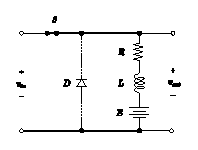
\includegraphics[width=\textwidth]{figuras/buck_converter_rle_s1.eps}
    \caption{1ª Etapa}
    \label{fig:buck_converter_rle_s1}
  \end{subfigure}
  \hfil
  \begin{subfigure}[t]{0.33\textwidth}
    \centering
    \includegraphics[width=\textwidth]{figuras/buck_converter_rle_s2.eps}
    \caption{2ª Etapa}
    \label{fig:buck_converter_rle_s2}
  \end{subfigure}
  \caption{Etapas de funcionamento do conversor Buck com carga RLE. As linhas tracejadas indicam que a corrente no ramo é nula.}
\end{figure}

% Buck: Filtros
A corrente proveniente da fonte que alimenta o conversor Buck tem uma natureza pulsante, o que resulta em dois inconvenientes significativos. Em primeiro lugar, a presença de um elevado conteúdo harmônico pode causar perturbações radioelétricas, potencialmente interferindo com equipamentos de comunicação e sinalização. Além disso, caso haja indutância em série com a fonte, mesmo que seja de natureza parasitária, no momento da abertura da chave, podem ser geradas sobretensões potencialmente destrutivas para os semicondutores de potência. Para superar essas dificuldades, recomenda-se a implementação de um filtro LC ou RLC, como ilustrado na \autoref{fig:buck_with_current_filter}. Em casos onde um conversor Buck precisa fornecer uma saída com uma tensão contínua de baixa ondulação, é essencial incluir um filtro passa-baixa composto por um indutor e um capacitor, conforme ilustrado na \autoref{fig:buck_with_voltage_filter}. \cite{martins2008}.

\begin{figure}[H]
  \captionsetup{justification=centering}
  \centering
  \begin{subfigure}[t]{0.45\textwidth}
    \centering
    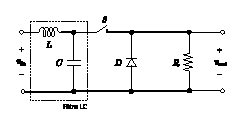
\includegraphics[width=\textwidth]{figuras/buck_with_current_filter.eps}
    \caption{Filtragem da corrente de entrada}
    \label{fig:buck_with_current_filter}
  \end{subfigure}
  \hfil
  \begin{subfigure}[t]{0.45\textwidth}
    \centering
    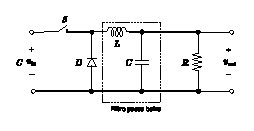
\includegraphics[width=\textwidth]{figuras/buck_with_voltage_filter.eps}
    \caption{Filtragem da tensão de saída.}
    \label{fig:buck_with_voltage_filter}
  \end{subfigure}
  \caption{Conversor Buck com filtros.}
\end{figure}

\subsection{Conversor Boost}

% Boost: Introdução
O conversor \acrshort{cc}-\acrshort{cc} de elevação de tensão, conhecido como conversor Boost, tem sua tensão média de saída teoricamente equivalente à tensão de alimentação. Embora sua estrutura utilize uma quantidade semelhante de componentes ao conversor Buck, estes são reorganizados para formar uma nova topologia. Essa configuração envolve a adição de uma indutância em série com a fonte de alimentação, transformando-a em uma fonte de corrente. Consequentemente, a carga deve ser projetada para se comportar como uma fonte de tensão, conforme as premissas estabelecidas anteriormente. \cite{martins2008}.

% Boost: Estrutura básica
A \autoref{fig:basic_boost_converter_a} apresenta a estrutura básica do conversor Boost. Em altas frequências de chaveamento, a corrente de entrada pode ser considerada constante, denotada por $i_{in}$, e o circuito pode ser representado conforme ilustrado na \autoref{fig:basic_boost_converter_b}. \cite{martins2008}.

\begin{figure}[h]
  \centering
  \captionsetup{justification=centering}
  \begin{subfigure}[b]{0.33\textwidth}
    \centering
    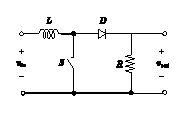
\includegraphics[width=\textwidth]{figuras/basic_boost_converter_a.eps}
    \caption{}
    \label{fig:basic_boost_converter_a}
  \end{subfigure}%
  \hfil
  \begin{subfigure}[b]{0.37\textwidth}
    \centering
    \includegraphics[width=\textwidth]{figuras/basic_boost_converter_b.eps}
    \caption{}
    \label{fig:basic_boost_converter_b}
  \end{subfigure}
  \caption{Estrutura básica do conversor Boost.}
  \label{fig:boost_converter}
\end{figure}

% Boost: relação tensão entrada-saída
Considerando que a chave $S$ opera com frequência fixa e duty cycle variável, podemos expressar a energia fornecida pela fonte de entrada $v_{in}$ como: \begin{equation} \mathcal{E}_{in} = v_{in} i_{in} T, \end{equation} E a energia recebida pela carga como: \begin{equation} \mathcal{E}_{out} = v_{out} i_{in} t_a. \end{equation} Portanto, a energia recebida pela carga é dada por: \begin{equation} \mathcal{E}_{out} = v_{out} i_{in} (T - t_c). \end{equation} Considerando o sistema conservativo, isto é, $\mathcal{E}_{in} = \mathcal{E}_{out}$, obtemos: \begin{equation} v_{in} i_{in} T = v_{out} i_{in} (T - t_c). \end{equation} Assim, \begin{equation} \frac{v_{out}}{v_{in}} = \frac{1}{1-d} \label{eq:ideal_feature_boost}.\end{equation} Esta última equação representa a característica ideal de transferência do conversor Boost. Quando o duty cycle $d$ tende a 1, $v_{out}$ tende ao infinito. Além disso, a tensão mínima de saída é igual à tensão de entrada $v_{in}$. \cite{martins2008}.

% Boost: relação corrente entrada-saída
A potência de entrada e saída são definidas da seguinte forma: \begin{align} P_{\text{in}} &= v_{\text{in}} \cdot i_{\text{md}} \\ P_{\text{out}} &= v_{\text{out}} \cdot i_{\text{out}}, \end{align} onde $i_{\text{md}}$ é a corrente média da entrada do conversor Boost. A partir destas equações e considerando que o conversor é conservativo, ou seja, $P_{\text{in}} = P_{\text{out}}$, tem-se: \begin{gather} v_{in} i_{\text{md}} = v_{\text{out}}i_{\text{out}} \\ \frac{i_{\text{out}}}{i_{md}} = \frac{v_{\text{in}}}{v_{\text{out}}} \label{eq:boost_converter_iv} \end{gather}

A partir das equações \eqref{eq:ideal_feature_boost} e \eqref{eq:boost_converter_iv}, a relação entre a corrente média de saída a corrente média de saída pode ser expressa como: \begin{equation} i_{\text{out}} = (1 - d) \cdot i_{\text{in}} \label{eq:boost_converter_current_transfer} \end{equation} e relação entre a tensão de entrada e tensão média de saída como: \begin{equation} v_{\text{out}} = \frac{1}{(1 - d)} \cdot v_{\text{in}}. \label{eq:boost_converter_voltage_transfer}\end{equation}

% Boost: Etapas de funcionamento
O conversor Boost, ilustrado na \autoref{fig:boost_converter}, opera em duas etapas distintas, descritas como segue: na fase inicial $(0, t_c)$, representada na \autoref{fig:boost_converter_s1}, o processo tem início com o fechamento da chave S. Nesse intervalo, o diodo D é polarizado inversamente, isolando o estágio de saída da fonte de alimentação $i_{in}$, que está em curto-circuito. A corrente na chave é equivalente à corrente da fonte de alimentação, enquanto a corrente no diodo D é nula. Essa fase é concluída quando a chave S é aberta. Na segunda etapa $(t_c, T)$, representada na \autoref{fig:boost_converter_s2}, ocorre a condução do diodo D quando a chave S é aberta, permitindo que a fonte de corrente $i_{in}$ entregue energia à carga. Durante esse período, a corrente na chave é nula, e a corrente no diodo D é igual à corrente da fonte de alimentação. O término dessa etapa ocorre com o fechamento da chave S, dando início novamente à primeira etapa. \cite{martins2008}.

\begin{figure}[h]
  \centering
  \captionsetup{justification=centering}
  \begin{subfigure}[b]{0.37\textwidth}
    \centering
    \includegraphics[width=\textwidth]{figuras/boost_converter_s1.eps}
    \caption{Primeira etapa.}
    \label{fig:boost_converter_s1}
  \end{subfigure}%
  \hfil
  \begin{subfigure}[b]{0.37\textwidth}
    \centering
    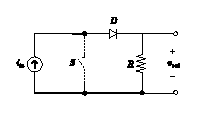
\includegraphics[width=\textwidth]{figuras/boost_converter_s2.eps}
    \caption{Segunda etapa.}
    \label{fig:boost_converter_s2}
  \end{subfigure}
  \caption{Etapas de funcionamento do conversor Boost. As linhas tracejadas indicam que a corrente é nulo no ramo.}
\end{figure}

% Boost: Capacitor em paralelo com a carga
Como visto anteriormente, a fonte de alimentação $V_{in}$, conectada em série com um indutor $L$, age como uma fonte de corrente. Portanto, a carga deve operar como uma fonte de tensão. Logo, se a carga for indutiva, é necessário conectar em paralelo a ela um capacitor de valor apropriado, conforme ilustrado na figura abaixo. \cite{martins2008}.

\begin{figure}[H]
  \centering
  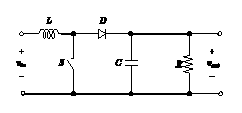
\includegraphics[width=0.5\textwidth]{figuras/boost_converter_capacitor.eps}
  \caption{Conversor Boost com capacitor em paralelo com a carga.}
  \label{fig:boost_converter_capacitor}
\end{figure}

\section{Modelagem Matemática}

% Modelagem: Introdução
Nesta seção, será discutida a modelagem matemática de conversores Buck e Boost conectados a uma \acrshort{cpl}. O conversor Buck reduz a tensão contínua de alta para baixa, enquanto o conversor Boost a eleva de baixa para alta. A \acrshort{cpl} demanda potência constante, independentemente da tensão de entrada. Desta forma, pode-se obter uma base sólida para análises subsequentes e o desenvolvimento de estratégias de \acrshort{etc}.

\subsection{Conversor Buck}

% Modelagem Buck: Apresentação do circuito
O sistema inicialmente utilizado neste estudo é um conversor constituído por um conversor Buck básico com filtro de tensão de saída $RLC$ conectado a uma \acrshort{cpl}. A \acrshort{cpl} é representada por um resistor e uma fonte de corrente dependente da potência da \acrshort{cpl}, conforme a seguinte equação: \begin{equation} i_{CPL}(t) = \frac{P_{CPL}(t)}{v_{out}(t)} \label{eq:cpl_current} \end{equation} onde $i_{CPL}(t)$ é a corrente da \acrshort{cpl} em função do tempo, a $P_{CPL}(t)$ é a potência da \acrshort{cpl} e $v_{out}(t)$ é a tensão de saída do conversor em função do tempo.

\begin{figure}[H]
  \centering
  \captionsetup{justification=centering}
  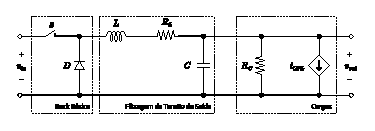
\includegraphics[width=0.87\textwidth]{figuras/buck_converter_circuit.eps}
  \caption{Circuito \textit{Buck} com \acrshort{cpl}.}
  \label{fig:circuit1}
\end{figure}

% Modelagem Buck: Corrente do indutor
Conforme abordado na \autoref{section:buck_converter}, a tensão fornecida pelo conversor Buck para o restante do circuito é igual ao produto entre a tensão de entrada $v_{in}$ e o duty cycle $d(t)$. Considerando esta característica e aplicando a \acrfull{lkt} no filtro, obtém-se a seguinte equação: \begin{equation} d(t)v_{in} - L \dt{i}_L - R_L i_L(t) - v_C(t) = 0, \end{equation} onde $i_L$ é corrente no indutor e $v_C$ é a tensão sobre o capacitor. Desta forma, é possível determinar a equação dinâmica da corrente do indutor, que é: \begin{equation} \dt{i}_L = - \frac{R_L}{L} i_L(t) - \frac{1}{L} v_C(t) + \frac{v_{in}}{L}d(t). \label{eq:buck_converter_current} \end{equation}

% Modelagem Buck: Tensão do capacitor
Por meio da \acrfull{lkc}, pode-se definir a corrente do indutor $i_{L}$ como a soma das correntes através do capacitor $C$, da resistência $R_C$ e da \acrshort{cpl}: \begin{equation} i_L(t) = i_C(t) + i_R(t) + i_{CPL}(t). \end{equation} Dessa forma, considerando $i_C(t) = C\dt{v}_C$, $i_R(t) = \frac{v_C(t)}{R_C}$ e $i_{CPL}(t)$ definida em \eqref{eq:cpl_current}, obtém-se: \begin{equation} i_L(t) = C\dt{v}_C + \frac{v_C(t)}{R_C} + \frac{P_{CPL}}{v_C(t)}. \end{equation} Logo, a equação dinâmica da tensão do capacitor é expressa por: \begin{equation} \dt{v}_C = \frac{1}{C} i_L(t) - \frac{1}{CR_C}v_C(t) - \frac{P_{CPL}}{Cv_C(t)} \label{eq:buck_converter_voltage} \end{equation}

% Modelagem Buck: Modelo não-linear
A partir das equações dinâmicas \eqref{eq:buck_converter_current} e \eqref{eq:buck_converter_voltage}, pode-se estabelecer o modelo dinâmico do sistema como segue: \begin{equation}\begin{cases} \dt{i}_L &=  - \frac{R_L}{L} i_L(t) - \frac{1}{L} v_C(t) + \frac{v_{in}}{L}d(t)  \\ \dt{v}_C &= \frac{1}{C} i_L(t) - \frac{1}{C R_C} v_C(t) - \frac{1}{C v_C(t)} P_{CPL}(t) \label{eq:buck_nonlinear_system} \end{cases}, \end{equation} onde $i_L(t)$ e $v_C(t)$ são os estados do sistema, e $d(t)$ e $P_{CPL}(t)$ são as entradas.

\subsection{Conversor Boost}

O segundo sistema utilizada neste estudo consiste em um conversor Boost conectado a uma \acrshort{cpl}, onde um capacitor é adicionado em paralelo, uma vez que a carga é considerada possuir características indutivas. A modelagem da \acrshort{cpl} segue a mesma metodologia do sistema anterior, representando-a por uma fonte de corrente dependente. A Figura \autoref{fig:boost_converter_cpl} ilustra o circuito completo deste sistema para a modelagem.

\begin{figure}[H]
  \centering
  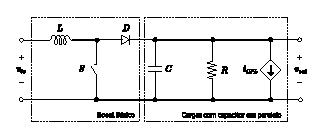
\includegraphics[width=.73\textwidth]{figuras/boost_converter_cpl.eps}
  \caption{Conversor Boost conectado a uma \acrshort{cpl}.}
  \label{fig:boost_converter_cpl}
\end{figure}

Por meio da relação entre a tensão de entrada e a tensão média de saída do conversor Boost, conforme descrito na equação \eqref{eq:boost_converter_voltage_transfer}, e da \acrshort{lkt}, obtém-se: \begin{equation} L \dt{i}_L - \frac{1}{1-d} v_{\text{in}} - v_c(t) = 0. \end{equation} Dessa forma, a equação dinâmica da corrente do indutor é expressa como: \begin{equation} \dt{i}_L = \frac{1}{L}v_{\text{in}} - \frac{1-d}{L}v_C(t) \label{eq:boost_converter_current}. \end{equation}

Ao aplicar a \acrshort{lkc}, temos que a corrente do diodo é igual à soma das correntes do capacitor, do resistor e da corrente $i_{CPL}(t)$, definida em \eqref{eq:cpl_current}. A corrente do diodo é igual à corrente média de saída do conversor Boost, expressa na equação \eqref{eq:boost_converter_current_transfer}. Portanto, \begin{equation} (1 - d) i_{\text{in}}(t) = C\dt{v}_C + \frac{v_C(t)}{R} + \frac{P_{CPL}(t)}{v_C(t)}.\end{equation} Considerando altas frequências de chaveamento, a corrente média de entrada pode ser considerada igual à corrente do indutor. Assim, a equação dinâmica da tensão do capacitor pode ser expressa como: \begin{equation} \dt{v}_C = \frac{1 - d}{C} i_L(t) - \frac{1}{RC}v_C(t) - \frac{1}{Cv_C(t)}P_{CPL}(t). \label{eq:boost_converter_voltage}\end{equation}

Desse modo, o modelo dinâmico médio do segundo sistema pode ser formulado a partir das equações \eqref{eq:boost_converter_current} e \eqref{eq:boost_converter_voltage}. Este modelo é representado por: \begin{equation} \begin{cases} \dt{i}_L(t) = - \frac{1-d(t)}{L}v_C(t) + \frac{1}{L}v_{in} \\ \dt{v}_C(t) = \frac{1 - d(t)}{C} i_L(t) - \frac{1}{RC}v_C(t) - \frac{1}{Cv_C(t)}P_{CPL}(t). \label{eq:boost_nonlinear_system}\end{cases} \end{equation} As grandezas $i_L(t)$ e $v_C(t)$ representam os estados do sistema. Enquanto que $d(t)$ e $P_{CPL}(t)$ representam as entadas do sistema, onde o duty cycle é controlável e a potência da \acrshort{cpl} é considerada a pertubação do sistema.

\subsection{Transladação dos modelos obtidos}

% Transladação: introdução
Para estudo dos sistemas dinâmicos em um ponto de equilíbrio \begin{equation} P_{\text{o}} = \left({i_L}_{\text{o}}, \, {v_C}_{\text{o}}, \, d_{\text{o}}, \, {P_{cpl}}_{\text{o}} \right). \label{eq:operation_point} \end{equation} Ambos os sistemas serão transladados pelo método de mudança de variáveis. As variáveis de estado e as entradas de ambos os sistemas serão decompostas em termos constantes (seus valores no ponto de equilíbrio) e variantes no tempo, conforme apresentado nas equações a seguir: \begin{align}
  {i_L}(t) & = {i_L}_o + \delta i_L(t), & {v_C}(t)     & = {v_C}_o + \delta v_C(t), \label{eq:tranlation_decomposed_states}        \\[12pt]
  {d}(t)   & = d_o + \delta d(t),       & {P_{cpl}}(t) & = {P_{cpl}}_o + \delta P_{cpl}(t) \label{eq:tranlation_decomposed_inputs}
\end{align} Da mesma forma, as derivadas temporais das variáveis de estado também são decompostas: \begin{align}
  \dt{i}_L = {\dt{i_L}}_o + \delta \dt{i_L}, \hspace{1cm}
  \dt{v}_C = {\dt{v}_C}_o + \delta \dt{v}_C
\end{align} Essa decomposição facilita a análise da estabilidade do ponto de equilíbrio $P_o$ e a obtenção de respostas lineares no entorno do ponto de equilíbrio.

% Transladação: regime permanente 
Sob condições de operação em regime permanente, em ambos os sistemas, no ponto de operação, a corrente do indutor e a tensão do capacitor são nulos, ou seja: \begin{equation} {i_L}_o = 0, \hspace{1cm} {v_C}_o = 0. \label{eq:translation_null}\end{equation} Com base nisso, pode-se obter as equações transladadas da corrente do indutor e da tensão do capacitor nos sistemas dinâmicos obtidos. Substituindo a relação descrita em \eqref{eq:translation_null} na equação da corrente $i_L$ no sistema dinâmico \eqref{eq:buck_nonlinear_system} no ponto de equilíbrio $P_o$, obtém-se: \begin{gather}
  - \frac{R_L}{L} {i_L}_o - \frac{1}{L} {v_C}_o + \frac{v_{in}}{L}  d_o = 0  \notag \\[12pt]
  - R_L {i_L}_o - {v_C}_o + v_{in}  d_o = 0 \notag \\[12pt]
  d_o = \frac{R_L}{v_{in}} {i_L}_o + \frac{{v_C}_o}{v_{in}} \label{eq:tranlation_buck_d_op}
\end{gather} Dado os valores da corrente do indutor e da tensão do capacitor, ambos no ponto de operação, é possível determinar o valor de operação do duty cycle $d_o$ por meio da relação expressa em \eqref{eq:tranlation_buck_d_op}. Substituindo as variáveis decompostas apresentadas em \eqref{eq:tranlation_decomposed_states} e \eqref{eq:tranlation_decomposed_inputs} na equação da corrente do $\dt{i}_L$ do primeiro sistema, obtém-se a sua forma transladada: \begin{gather}
  {\dot{i_L}}_o + \delta \dot{i_L}_ = - \frac{R_L}{L} \left({i_L}_o + \delta i_L(t)\right) - \frac{1}{L} \left({v_C}_o + \delta v_C(t)\right) + \frac{v_{in}}{L} \left(d_o + \delta d(t)\right) \notag\\[12pt]
  \delta \dot{i_L} = - \frac{R_L}{L} {i_L}_o - \frac{R_L}{L} \delta i_L - \frac{1}{L} {v_C}_o - \frac{1}{L} \delta v_C + \frac{v_{in}}{L} d_o + \frac{v_{in}}{L} \delta d \label{eq:translation_buck_current}
\end{gather} Por meio da relação expressa em \eqref{eq:tranlation_buck_d_op}, a equação \eqref{eq:translation_buck_current} pode ser simplificada como demonstrado a seguir: \begin{gather}
  \delta \dot{i_L} = - \frac{R_L}{L} {i_L}_o - \frac{R_L}{L} \delta i_L - \frac{1}{L} {v_C}_o - \frac{1}{L} \delta v_C +  \frac{R_L}{L} {i_L}_o + \frac{1}{L} {v_C}_o + \frac{v_{in}}{L} \delta d \notag \\[12pt]
  \delta \dot{i_L} = - \frac{R_L}{L} \delta i_L - \frac{1}{L} \delta v_C  + \frac{v_{in}}{L} \delta d \label{eq:translation_buck_current_simplified}
\end{gather}

Da mesma forma, a fim de transpor a equação de tensão do capacitor $\dt{v}_C$ do primeiro sistema \eqref{eq:buck_converter_voltage}, foi realizada uma análise no ponto de operação $P_o$, resultando na seguinte relação: \begin{gather}
  - \frac{1}{C R_C} {v_C}_o + \frac{1}{C} {i_L}_o - \frac{1}{C {v_C}_o} {P_{CPL}}_o = 0 \notag \\[12pt]
  - \frac{1}{R_C} {v_C}_o + {i_L}_o - \frac{1}{{v_C}_o} {P_{CPL}}_o = 0 \notag
\end{gather} \begin{equation}{i_L}_o = \frac{1}{R_C} {v_C}_o + \frac{1}{{v_C}_o} {P_{CPL}}_o \label{eq:translation_buck_iL_op}\end{equation} Assim, dado os valores da tensão de capacitor e a potência \acrshort{cpl}, ambos no ponto de operação, é possível determinar a corrente do indutor no ponto de operação por meio da relação obtida expressa em \eqref{eq:translation_buck_iL_op}. Substituindo as variáveis decompostas definidas em \eqref{eq:tranlation_decomposed_states} e \eqref{eq:tranlation_decomposed_inputs} na equação da tensão do capacitor do primeiro sistema \eqref{eq:buck_converter_voltage}, obtém-se: \begin{equation}
  \delta \dt{v}_C = - \frac{1}{C R_C} {v_C}_o - \frac{1}{C R_C} \delta v_C + \frac{1}{C} {i_L}_o + \frac{1}{C}  \delta i_L - \frac{1}{C \left({v_C}_o + \delta v_C\right)} \left({P_{cpl}}_o + \delta P_{cpl}\right) \label{eq:translation_buck_voltage}
\end{equation} Por meio da relação obtida expressa em \eqref{eq:translation_buck_iL_op}, a equação \eqref{eq:translation_buck_voltage} pode ser simplificada como demonstrado a seguir: \begin{gather}
  \delta \dt{v}_C = - \frac{1}{C R_C} {v_C}_o - \frac{1}{C R_C} \delta v_C + \frac{1}{C} \left(\frac{{v_C}_o}{R_C} + \frac{{P_{cpl}}_o}{{v_C}_o}\right) + \frac{1}{C}  \delta i_L - \frac{{P_{cpl}}_o + \delta P_{cpl}}{C \left({v_C}_o + \delta v_C\right)} \notag \\[12pt]
  \delta \dt{v}_C = - \frac{1}{C R_C} \delta v_C + \frac{1}{C {v_C}_o} {P_{cpl}}_o + \frac{1}{C}  \delta i_L - \frac{1}{C \left({v_C}_o + \delta v_C\right)} \left({P_{cpl}}_o + \delta P_{cpl}\right) \notag \\[12pt]
  \delta \dt{v}_C = - \frac{1}{C R_C} \delta v_C  + \frac{1}{C}  \delta i_L + \frac{{P_{cpl}}_o \delta v_C - {v_C}_o \delta P_{cpl}}{C {v_C}_o \left({v_C}_o + \delta v_C\right)}
\end{gather}

Portanto, o sistema transladado do primeiro sistema, em torno do ponto de operação $P_o$, é: \begin{equation}
  \begin{cases}
    \displaystyle \delta \dot{i_L} = - \frac{R_L}{L} \delta i_L - \frac{1}{L} \delta v_C  + \frac{v_{in}}{L} \delta d \\[12pt]
    \displaystyle \delta \dt{v}_C = - \frac{1}{C R_C} \delta v_C  + \frac{1}{C}  \delta i_L + \frac{{P_{cpl}}_o \delta v_C - {v_C}_o \delta P_{cpl}}{C {v_C}_o \left({v_C}_o + \delta v_C\right)}
    \label{eq:translated_nonlinear_buck}
  \end{cases}
\end{equation}

Do mesmo modo que foi realizado o processo de translação para o primeiro sistema, o mesmo foi aplicado ao segundo sistema \eqref{eq:boost_nonlinear_system}. No ponto de operação $P_o$, pode-se obter a seguinte relação: \begin{gather}
  - \frac{1 - d_o}{L}{v_C}_o + \frac{1}{L}v_{in} = 0 \notag \\[12pt]
  {d}_o = 1 - \frac{v_{in}}{{v_C}_o} \label{eq:translation_boost_d_op},
\end{gather} Logo, por meio desta relação, é possível determinar o duty cycle no ponto de operação dado o valor da tensão do capacitor também no ponto de operação. Reescrevendo a equação da corrente do segundo sistema, expressa em \eqref{eq:boost_converter_current}, substituindo as variáveis descritas em \eqref{eq:tranlation_decomposed_states} e \eqref{eq:tranlation_decomposed_inputs}, obtém-se: \begin{gather}
  \dt{\delta i_L}  = - \frac{1 - (d_o + \delta d) }{L} ({v_C}_o + \delta v_C) + \frac{1}{L} v_{in} \label{eq:translation_boost_current}
\end{gather} Substituindo a relação \eqref{eq:translation_boost_d_op} na equação \eqref{eq:translation_boost_current}, pode-se obter a sua forma simplificada: \begin{gather}
  \dt{\delta i_L}  = - \frac{1 - (1 - \displaystyle \frac{v_{in}}{{v_C}_o} + \delta d) }{L} ({v_C}_o + \delta v_C) + \frac{1}{L} v_{in} \notag  \\[12pt]
  \dt{\delta i_L}  = - \frac{\displaystyle \frac{v_{in}}{{v_C}_o} - \delta d }{L} ({v_C}_o + \delta v_C) + \frac{1}{L} v_{in} \notag  \\[12pt]
  \dt{\delta i_L}  = - \frac{v_{in}}{L{v_C}_o}\delta v_C + \left(\frac{{v_C}_o + \delta {v_C}}{L}\right) \delta d
\end{gather}

No ponto de operação $P_o$ do segundo sistema, da equação que descreve a tensão do capacitor $\dt{v}_C$, expressa em \eqref{eq:boost_converter_voltage}, pode-se obter a próxima relação do segundo sistema: \begin{gather}
  0 = \frac{1 - d_o}{C} {i_L}_o - \frac{1}{RC}{v_C}_o - \frac{1}{C{v_C}_o}{P_{cpl}}_o \notag \\[12pt]
  (1 - d_o){i_L}_o - \frac{1}{R}{v_C}_o - \frac{1}{{v_C}_o}{P_{cpl}}_o = 0 \notag \\[12pt]
  {i_L}_o = \frac{{v_C}_o}{R(1-d_o)} + \frac{{P_{cpl}}_o}{{v_C}_o (1 - d_o)} \notag \\[12pt]
  {i_L}_o = \frac{{v_C}^2_o + R{P_{cpl}}_o}{R{v_C}_o(1 - d_o)}
\end{gather} Por meio da relação \eqref{eq:translation_boost_d_op}, a equação anterior pode ser simplificada para: \begin{equation}
  {i_L}_o = \frac{{v_C}^2_o + R{P_{cpl}}_o}{R{v_{in}}}
  \label{eq:translation_boost_iL_op}
\end{equation} Dessa forma, tendo a tensão do capacitor e a potência da \acrshort{cpl} no ponto de operação, é possível determinar a corrente nesse ponto, utilizando a relação estabelecida em \eqref{eq:translation_boost_iL_op}. Por fim, ao realizar as substituições das variáveis decompostas conforme definidas em \eqref{eq:tranlation_decomposed_inputs} e \eqref{eq:tranlation_decomposed_states}, é obtida a forma transladada da equação da tensão $\dt{v}_C$ do segundo sistema definida em \eqref{eq:boost_converter_voltage}: \begin{gather}
  {{\dt{v}_C}}_o + \dt{\delta {v}_C} = \frac{1 - (d_o + \delta d)}{C} ( {i_L}_o + \delta i_L) - \frac{{v_C}_o + \delta v_C}{RC} - \frac{{{P_{cpl}}_o + \delta P_{cpl}}}{C({v_C}_o + \delta {v_C})}
\end{gather}

Simplificando por meio das relações expressas em \eqref{eq:translation_boost_d_op} e \eqref{eq:translation_boost_iL_op}, obtém-se: \begin{gather}
  \dt{\delta {v}_C} = \left( \frac{1 - d_o}{C} - \frac{\delta d}{C} \right)\left({i_L}_o + \delta i_L\right) - \frac{{v_C}_o + \delta v_C}{RC} - \frac{{{P_{cpl}}_o + \delta P_{cpl}}}{C({v_C}_o + \delta {v_C})}
\end{gather}

\subsection{Linearização dos modelos obtidos}

% Linearização - introdução
Por causa da presença de não linearidades em ambos os modelos, \eqref{eq:buck_nonlinear_system} e \eqref{eq:boost_nonlinear_system}, eles são intrinsecamente não lineares. Para abordar essa não linearidade, pode-se linearizá-los, obtendo um conjunto de equações que descrevem pequenas mudanças em torno do ponto de equilíbrio $P_{\text{eq}}$ nos estados dos sistemas, $i_L(t)$ e $v_C(t)$.

% Linearização - sistema linearizado genérico
A linearização é feita por meio da aproximação de primeira ordem da série de Taylor em torno do ponto de equilíbrio $P_{\text{eq}} = ({i_L}_{\text{eq}}, \, {v_C}_{\text{eq}}, \, {d}_{\text{eq}}, \, {P_{CPL}}_{\text{eq}})$, conforme descrito a seguir: \begin{gather}  \dt{\delta i_L} = \frac{\partial \dt{i}_L}{\partial i_L}\delta i_L(t) + \frac{\partial \dt{i}_L}{\partial v_C}\delta v_C(t) + \frac{\partial {\dt{i}_L}}{\partial d}\delta d(t) + \frac{\partial {\dt{i}_L}}{\partial P_{CPL}}\delta P_{CPL}(t) \\ \nonumber \\ \dt{\delta v_C} = \frac{\partial \dt{v}_C}{\partial i_L}\delta i_L(t) + \frac{\partial \dt{v}_C}{\partial v_C}\delta v_C(t) + \frac{\partial \dt{v}_C}{\partial d}\delta d(t) + \frac{\partial \dt{v}_C}{\partial P_{CPL}}\delta P_{CPL}(t), \end{gather} onde, o símbolo $\delta$ indica a variação da variável em relação ao ponto de equilíbrio, isto é, \begin{equation} \delta f(t) = f(t) - f_{\text{op}}. \label{eq:delta}\end{equation}

% Linearização - conversor buck
A partir dessas equações, podemos derivar as expressões linearizadas de $\dt{i}_L$ e $\dt{v}_C$ para o primeiro sistema, como mostrado abaixo: \begin{equation} \begin{cases} \delta \dt{i}_L &= -\frac{R_L}{L} \delta i_L(t) - \frac{1}{L} \delta v_C(t) + \frac{v_{\text{in}}}{L} \delta d(t) \\ \delta \dt{v}_C &= \frac{1}{C} \delta i_L(t) + \frac{1}{C} \left(\frac{{P_{CPL}}_{\text{eq}}}{{v_C}^2_{\text{eq}}} - \frac{1}{R_C}\right) \delta v_C(t) - \frac{1}{C{v_C}_{\text{eq}}} \delta P_{CPL}(t), \end{cases} \end{equation} ou, na forma de espaço de estados: \begin{equation} \begin{bmatrix} \dt{\delta i_L} \\ \dt{\delta v_C} \end{bmatrix} = \begin{bmatrix} \displaystyle -\frac{R_L}{L} & \displaystyle -\frac{1}{L}  \\\\ \displaystyle \frac{1}{C} & \displaystyle \frac{1}{C}\left(\frac{{P_{CPL}}_{\text{eq}}}{{{v_{C}}^2_{\text{eq}}}} - \frac{1}{R_C}\right) \end{bmatrix} \begin{bmatrix} \delta i_L(t) \\ \delta v_C(t) \end{bmatrix} + \begin{bmatrix} {\displaystyle \frac{v_{in}}{L}} & 0 \\ \\ 0 & \displaystyle {-\frac{1}{C{v_C}_{\text{eq}}}} \end{bmatrix}  \begin{bmatrix} \delta d(t) \\ \delta P_{CPL}(t) \end{bmatrix}. \label{eq:buck_linear_system}\end{equation}

Para o segundo modelo dinâmico \eqref{eq:boost_nonlinear_system}, têm-se: \begin{equation} \begin{cases} \delta \dt{i}_L &= - \frac{1 - d_{\text{eq}}}{L} \delta v_C(t) + \frac{{v_C}_{\text{eq}}}{L}\delta d(t) \\ \delta \dt{v}_C &= \frac{1 - d_{\text{eq}}}{C} \delta i_L(t) + \frac{1}{C} \left(\frac{{P_{CPL}}_{\text{eq}}}{{v_C}^2_{\text{eq}}} - \frac{1}{R}\right) \delta v_C(t) - \frac{{i_L}_{\text{eq}}}{C} \delta d(t) - \frac{1}{C{v_C}_{\text{eq}}} \delta P_{CPL}(t), \end{cases} \end{equation} ou, expresso na forma de espaço de estados: \begin{equation} \begin{bmatrix} \dt{\delta i_L} \\ \dt{\delta v_C} \end{bmatrix} = \begin{bmatrix} \displaystyle 0 & \displaystyle -\frac{1 - d_{\text{eq}}}{L}  \\\\ \displaystyle \frac{1 - d_{\text{eq}}}{C} & \displaystyle \frac{1}{C}\left(\frac{{P_{CPL}}_{\text{eq}}}{{{v_{C}}^2_{\text{eq}}}} - \frac{1}{R}\right) \end{bmatrix} \begin{bmatrix} \delta i_L(t) \\ \delta v_C(t) \end{bmatrix} + \begin{bmatrix} {\displaystyle \frac{{v_C}_{\text{eq}}}{L}} & 0 \\ \\ - \frac{{i_L}_{\text{eq}}}{C} & \displaystyle {-\frac{1}{C{v_C}_{\text{eq}}}} \end{bmatrix}  \begin{bmatrix} \delta d(t) \\ \delta P_{CPL}(t) \end{bmatrix}. \label{eq:boost_linear_system}\end{equation}

\section{Simulação}

Nesta seção, será realizada uma análise dos dois conversores \acrshort{cc}-\acrshort{cc} em malha aberta, analisando suas respostas em diversos cenários e condições operacionais. Utilizou-se a linguagem de programação Python juntamente com bibliotecas especializadas em simulação de sistemas dinâmicos para simular os modelos não-lineares transladados e os linearizados dos conversores obtidos na seção anterior. Com base nos resultados obtidos, é possível observar a influência de fatores como a variação das entradas e das condições de operação nos comportamentos dos conversores.

\subsection{Conversor Buck}

Dois modelos dinâmicos do conversor Buck, com os mesmos parâmetros de circuito, mas com pontos de operação distintos, foram utilizados para a análise em malha aberta. Cada conversor foi analisado utilizando o seu modelo não linear na forma transladada \eqref{eq:translated_nonlinear_buck} e o modelo linearizado \eqref{eq:buck_linear_system}. Os parâmetros do circuito, comuns aos dois modelos, estão detalhados na \autoref{table:circuit_parameter_buck}.

\vspace{8pt}
\begin{table}[H]
  \centering
  \begin{tabular}{cccc}
    \toprule
    Parâmetros & Símbolo  & Valor & Unidade \\
    \midrule
    Tensão de entrada & $v_{\mathrm{in}}$ & 48,00 & V \\
    Resistência de enrolamento do indutor & $r_L$ & 0,10 & $\Omega$ \\
    Carga de Resistência Constante & $r_{C}$ & 20,00 & $\Omega$ \\
    Indutância & $L$ & 1,00 & mH \\
    Capacitância  & $C$ & 2,20 & mC \\
    \bottomrule
  \end{tabular}
  \caption{Parâmetros do circuito do conversor Buck.}
  \label{table:circuit_parameter_buck}
\end{table}

A \autoref{table:op_parameters_buck} apresenta os pontos de operação de cada modelo do conversor Buck ("Buck 1" e "Buck 2"). Nesses pontos, a potência da carga e a tensão do capacitor são definidas, enquanto a corrente do indutor e o \textit{duty cycle} são calculados a partir da tensão do capacitor e da potência da carga, utilizando as equações \eqref{eq:translation_buck_iL_op} e \eqref{eq:tranlation_buck_d_op}, respectivamente.

\vspace{8pt}
\begin{table}[H]
  \centering
  \setlength{\tabcolsep}{10pt}
  \begin{tabular}{cccccc}
    \toprule
    \multirow{2}{*}{\centering Parâmetros} & \multirow{2}{*}{\centering Símbolo} & \multicolumn{2}{c}{\centering Valor} & \multirow{2}{*}{\centering Unidade} \\
    \cmidrule{3-4}
     &  & Buck 1 & Buck 2 &  \\
    \midrule
    Potência da \acrshort{cpl} & ${P_{\mathrm{cpl}}}_o$ & 50,00  & 250,00 & W \\
    Tensão do capacitor & ${v_C}_{\mathrm{o}}$ & 28,00 & 28,00  & V \\
    Corrente do indutor & ${i_L}_{\mathrm{o}}$ & 3,19 & 10,33 & A \\
    \textit{Duty cycle} & $d_{\mathrm{o}}$ & 0,58 & 0,60 & - \\  
    \bottomrule
  \end{tabular}
  \caption{Pontos de operação do dois modelos do conversor Buck.}
  \label{table:op_parameters_buck}
\end{table}

Por fim, o período de simulação é de 0 a 100 milissegundos. No primeiro modelo, a variação da corrente do indutor no instante inicial $\delta i_{L}(0)$ é de $-0,32 \textrm{ A}$  e a variação da tensão do capacitor $\delta v_{C}(0)$ é de $-1,40 \textrm{ V}$. No segundo modelo,  $\delta i_{L}(0) = -0,18 \textrm{ A}$ e  $\delta v_{C}(0) = -1,40 \textrm{ V}$.

\subsubsection{Sinais de Entrada Constantes}

A primeira simulação consiste em manter os parâmetros de entrada do sistema constantes, definindo-os como seus valores no \acrshort{po}. Isso resulta em variação nula em torno do \acrshort{po}, permitindo a análise do comportamento do conversor nesse estado. Os resultados para ambos os modelos do conversor Buck estão nas Figuras \ref{fig:simulation_1_buck_1} e \ref{fig:simulation_1_buck_2}. Nos gráficos apresentados na \autoref{fig:simulation_1_buck_1}, o modelo demonstra estabilidade, com a corrente do indutor e a tensão do capacitor convergindo rapidamente para seus valores no \acrshort{po}. Não há diferença significativa entre os modelos não linear e linearizado, validando a precisão deste último na representação do sistema.

\begin{figure}[H]
  \centering
  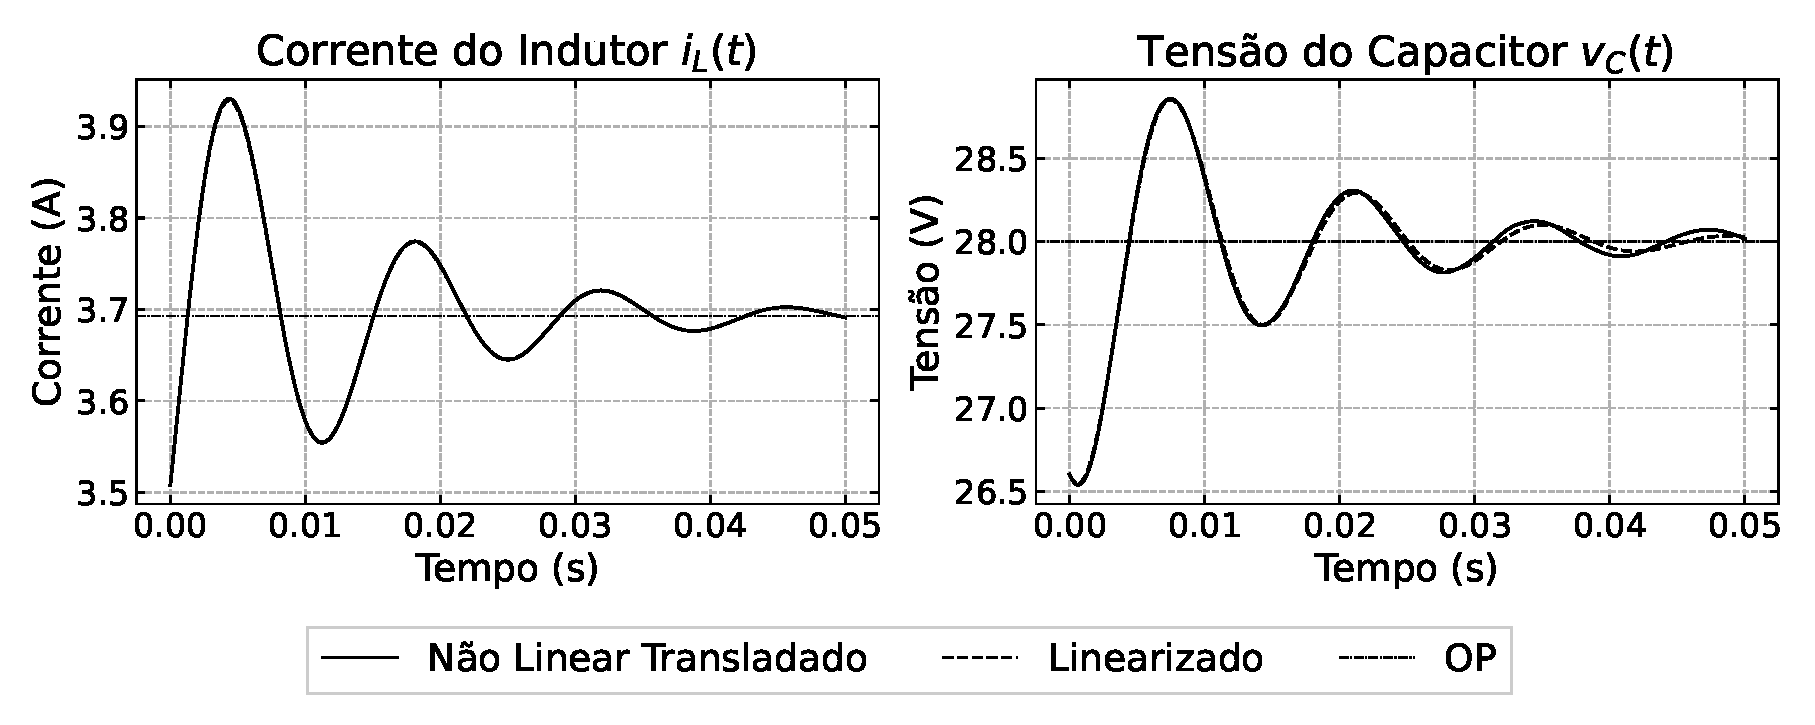
\includegraphics[width=1.\textwidth]{figuras/buck/simulation_1.eps}
  \caption{Simulação do primeiro modelo do conversor Buck com entradas constantes.}
  \label{fig:simulation_1_buck_1}
\end{figure}

No segundo modelo, no entanto, tanto a corrente do indutor quanto a tensão do capacitor apresentam um aumento gradativo e não se estabilizam, conforme mostrado na \autoref{fig:simulation_1_buck_2}. Portanto, o segundo modelo não converge para um estado estacionário, o que indica instabilidade. Ademais, o modelo linearizado apresentou grande precisão, sem diferenças significativa.

\begin{figure}[H]
  \centering
  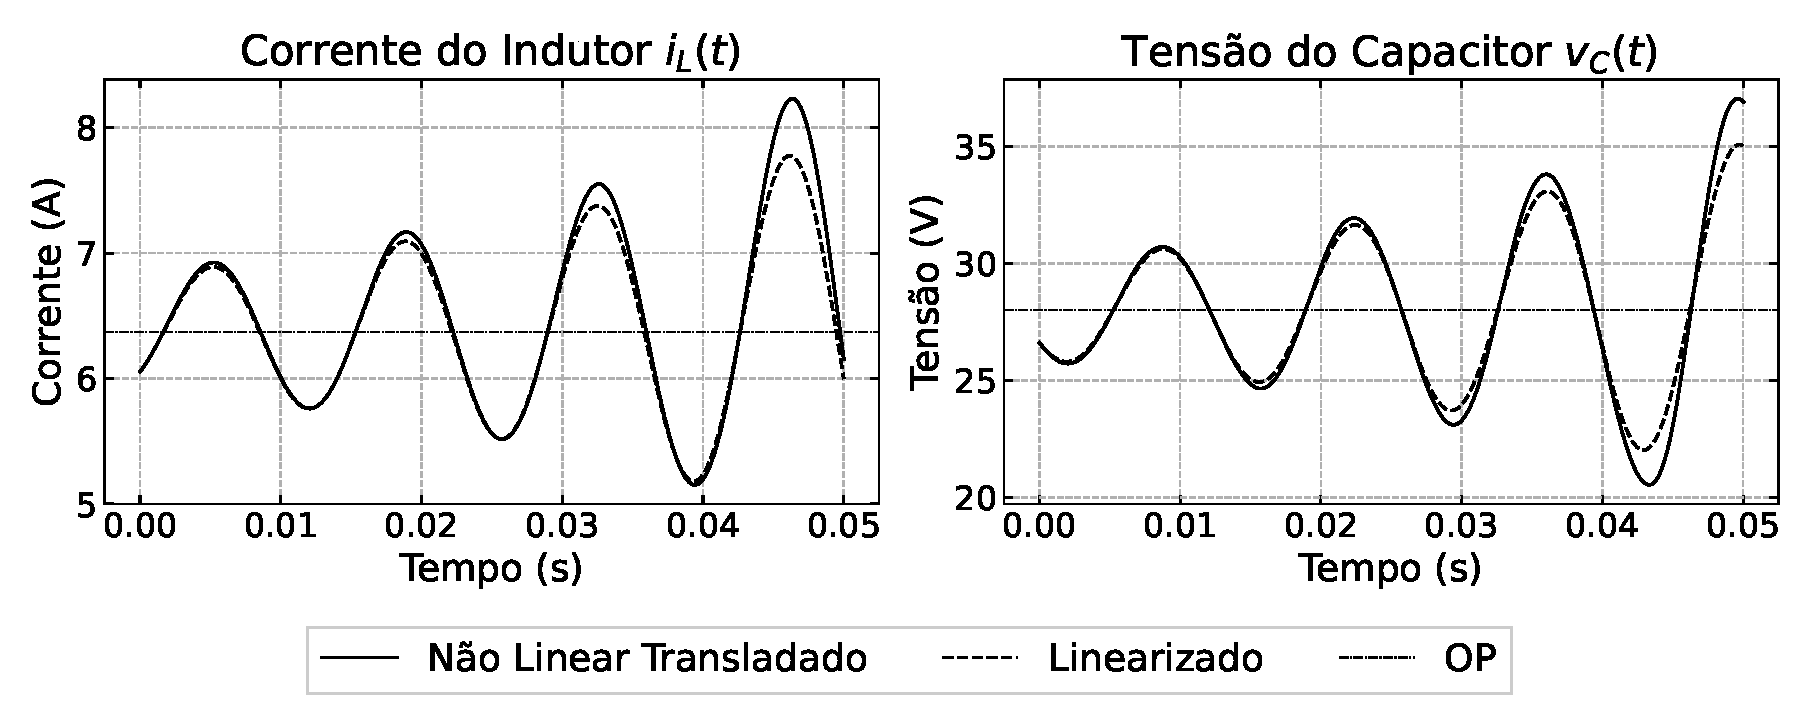
\includegraphics[width=1.\textwidth]{figuras/buck/simulation_2.eps}
  \caption{Simulação do segundo modelo do conversor Buck com entradas constantes.}
  \label{fig:simulation_1_buck_2}
\end{figure}

\subsubsection{Sinal de pertubação $P_{\textrm{cpl}}$ variável}



\subsection{Conversor Boost}

\subsubsection{Sinais de Entrada Constantes}

\subsubsection{Sinal de pertubação $P_{\textrm{cpl}}$ variável}